\begin{frame}[t, c]{A gallery of fluid examples}{Illustrative examples}
	\vspace{-0.5cm}
  \begin{minipage}{.64\textwidth}
    \centering
		\movie[width=\textwidth, autostart, loop]{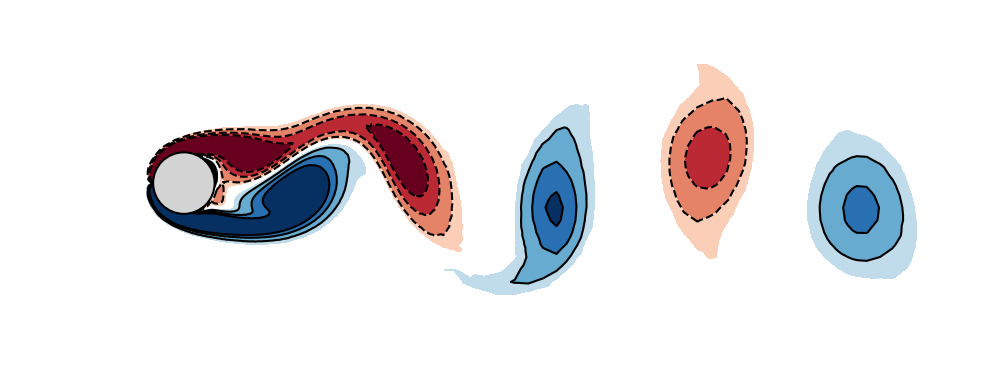
\includegraphics[width=\textwidth]{snapshot_re125_0}}{imgs/re125.mp4} \\

		Aerodynamics

		\medskip

		\movie[width=\textwidth, autostart, loop]{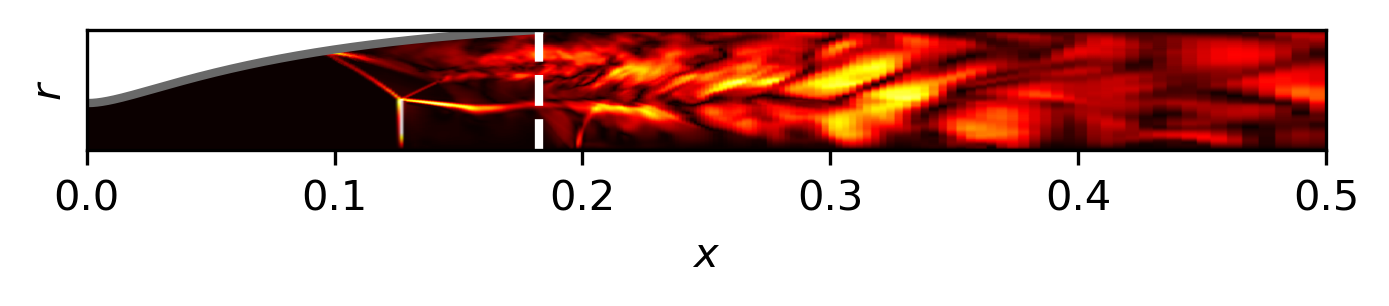
\includegraphics[width=\textwidth]{tic_m=1_fourier_mode_snapshot}}{imgs/tic_m=1_evolution.mp4} \\

		Rocket Science (litterraly!)
  \end{minipage}%
  \hfill
  \begin{minipage}{.32\textwidth}
    \centering
    \movie[width=\textwidth, autostart, loop]{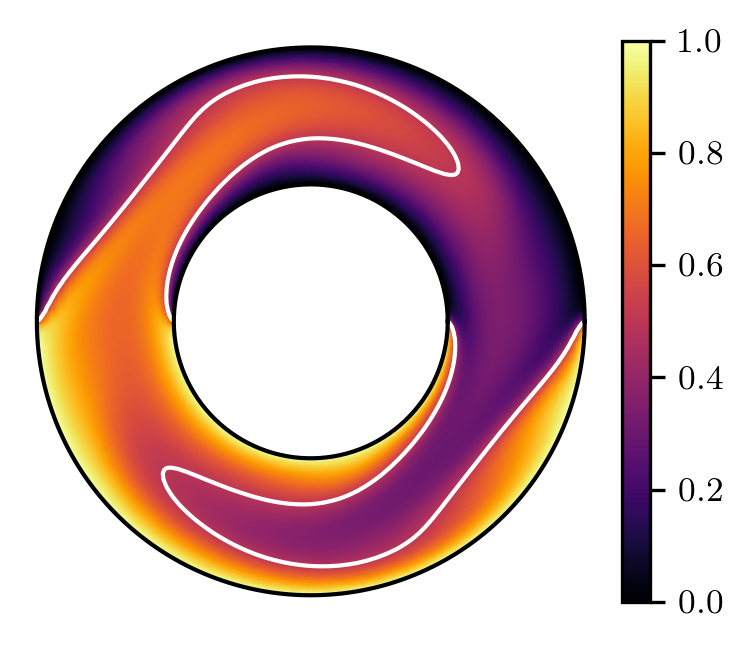
\includegraphics[width=\textwidth]{temperature_field_00000}}{imgs/temperature_evolution.mp4} \\

		Heat exchange
  \end{minipage}

\end{frame}

\begin{frame}[t, c]{A gallery of fluid examples}{Machine learning for physical systems}

	\centering
	\includegraphics[width=.8\textwidth]{physics_machine_learning}

	\vspace{1cm}
\end{frame}

\begin{frame}[t, c]{A gallery of fluid examples}{Low-order models}
	\begin{minipage}{.58\textwidth}
		\begin{itemize}
			\item Models can come in a lot of different flavors.

			\medskip

			\item Wiener proposed the following classification
			\begin{itemize}
				\item[\( \hookrightarrow	\)] \textbf{Black box:} input-output data.
				\item[\( \hookrightarrow	\)] \textbf{White box:} Input-output + known model.
				\item[\( \hookrightarrow	\)] \textbf{Gray box:} Input-output + partial knowledge of the model / inductive biases.
			\end{itemize}

			\medskip

			\item In physics, we are often in the third class.
			\begin{itemize}
				\item[\( \hookrightarrow	\)] Exact form of the equations may be unknown.
				\item[\( \hookrightarrow	\)] Knowledge of symmetries or invariants.
			\end{itemize}
		\end{itemize}
	\end{minipage}%
	\hfill
	\begin{minipage}{.38\textwidth}
		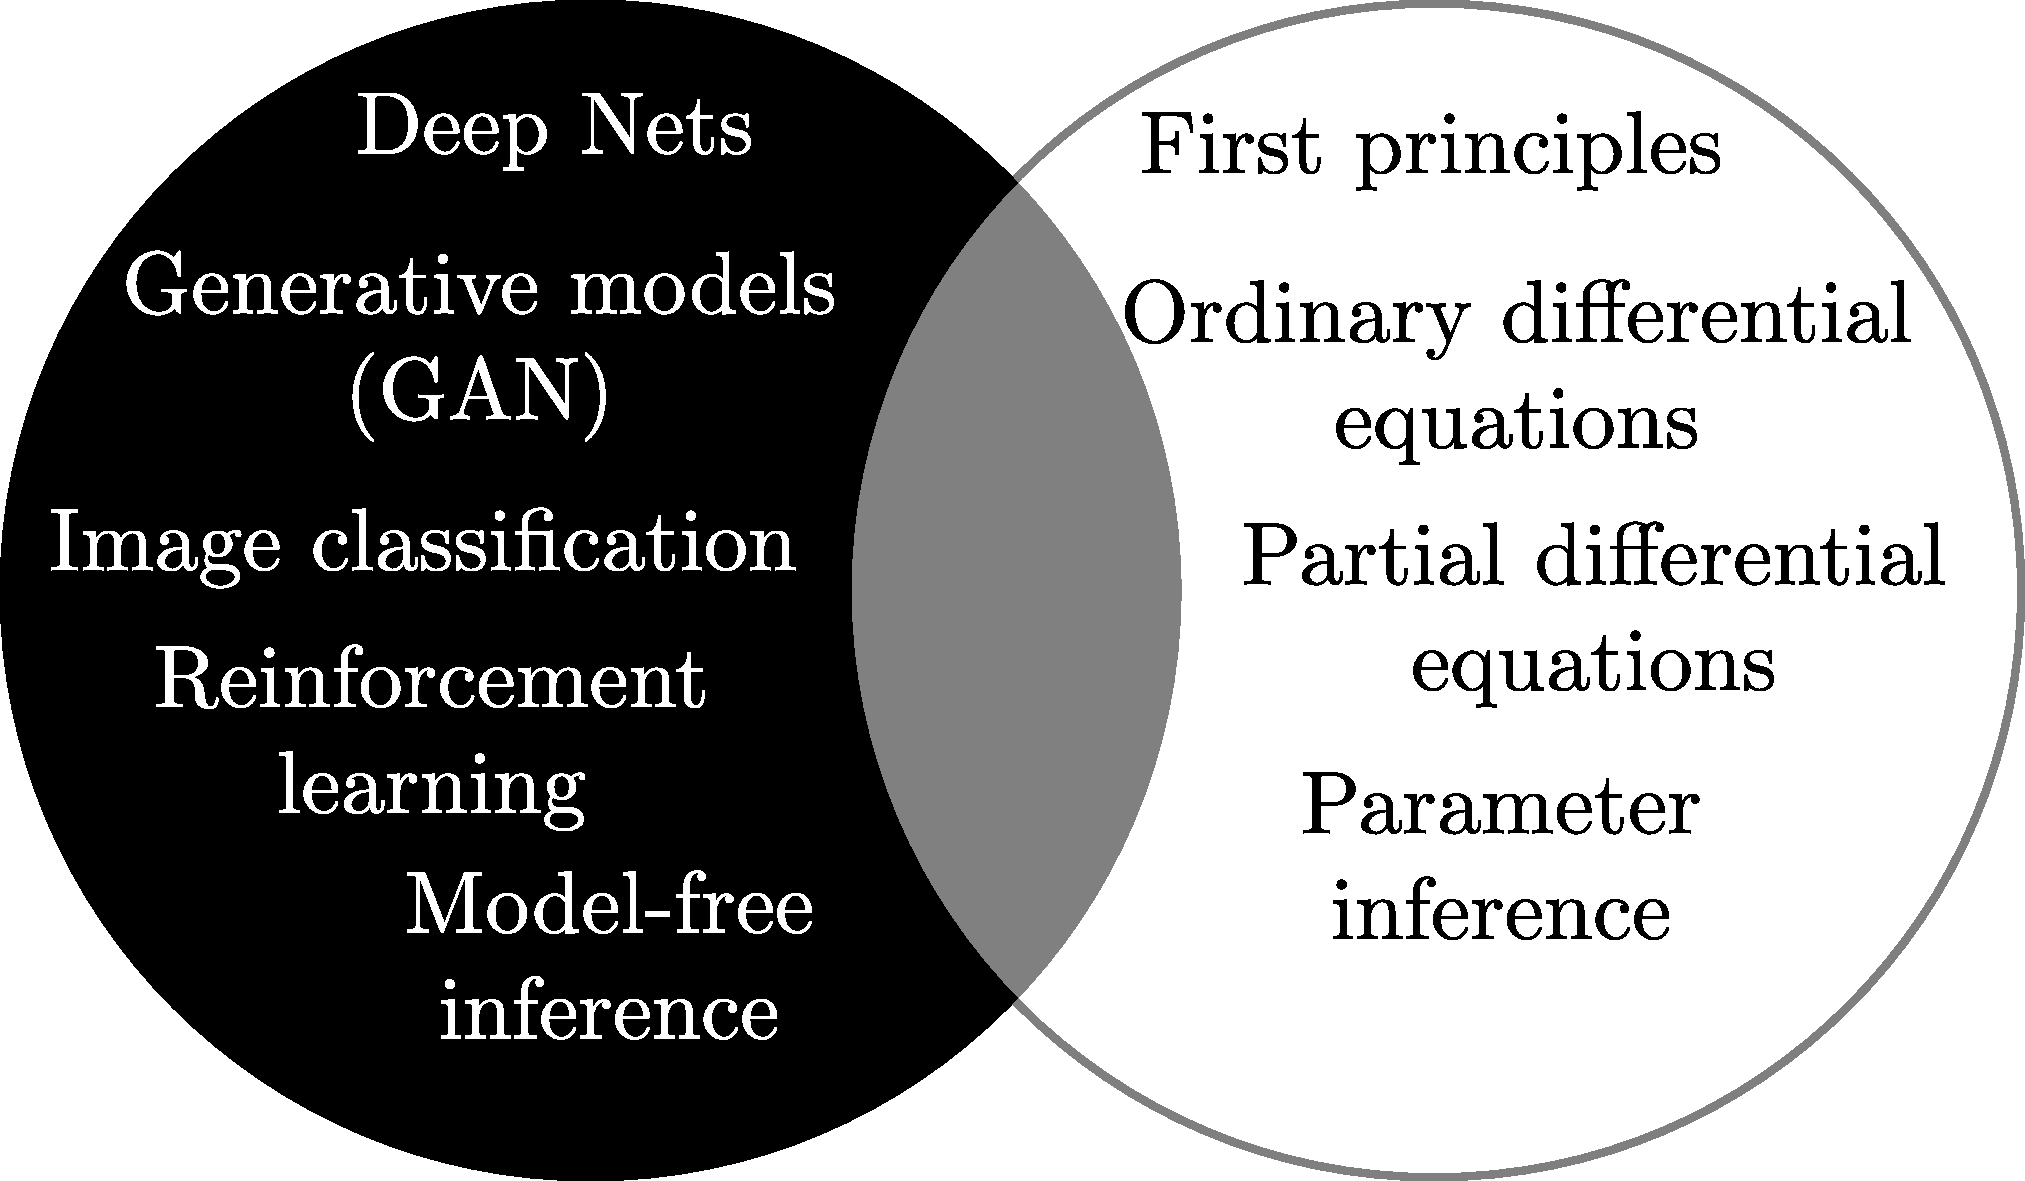
\includegraphics[width=\textwidth]{general_overview}
	\end{minipage}

	\vspace{1cm}
\end{frame}


\begin{frame}[t, c]{A gallery of fluid examples}{A prototypical example}

	\centering
	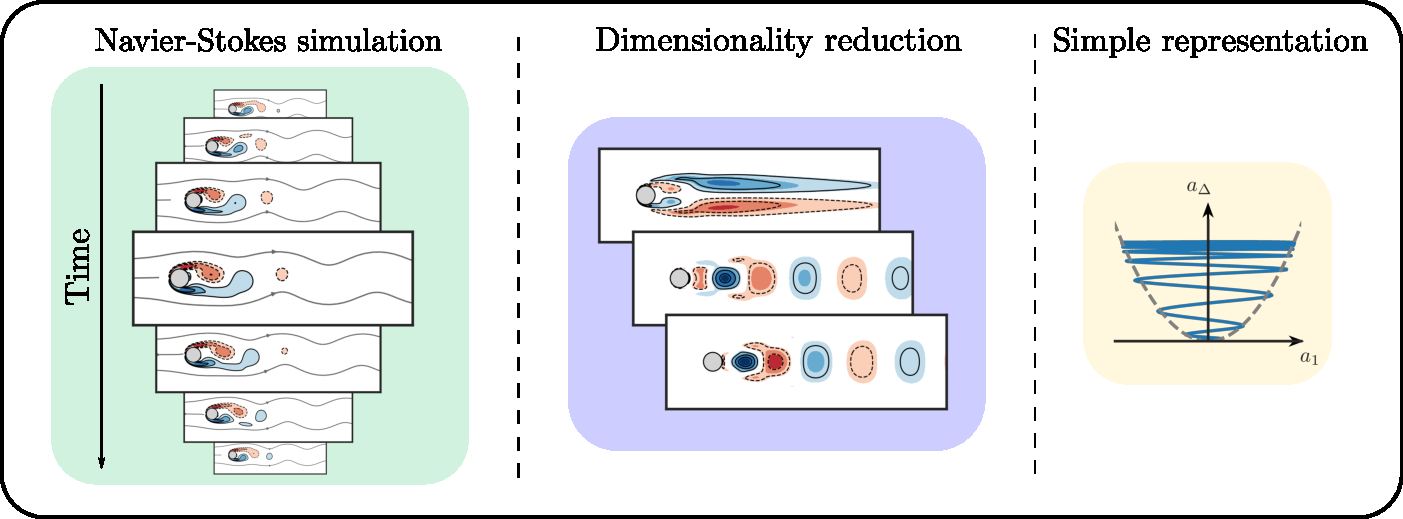
\includegraphics[width=.9\textwidth]{reduced_order_modeling}

	\vspace{1cm}
\end{frame}

\begin{frame}[t, c]{A gallery of fluid examples}{Low-order \underline{deterministic} models}
	\begin{minipage}{.58\textwidth}

		\begin{block}{}
			\textbf{Aim :} Identify an \underline{interpretable} and \underline{physically-consistent} low-order model.
		\end{block}

		\medskip

		\begin{itemize}
			\item Using \emph{SINDy}, the following model can be identified.
			%
			\[
				\begin{aligned}
					\dot{a}_1 & = \sigma a_1 - \omega a_2 - \alpha (a_1^2 + a_2^2) a_1 - \beta (a_1^2 + a_2^2) a_2 \\
					\dot{a}_2 & = \omega a_1 + \sigma a_2 + \beta (a_1^2 + a_2^2) a_1 - \alpha (a_1^2 + a_2^2) a_1.
				\end{aligned}
			\]

			\item \textbf{Interpretability :} Normal form of a supercritical Andronov-Poincaré-Hopf bifurcation.

			\item \textbf{Physical-consistency :} By design.
		\end{itemize}
	\end{minipage}%
	\hfill
	\begin{minipage}{.38\textwidth}
		\centering
		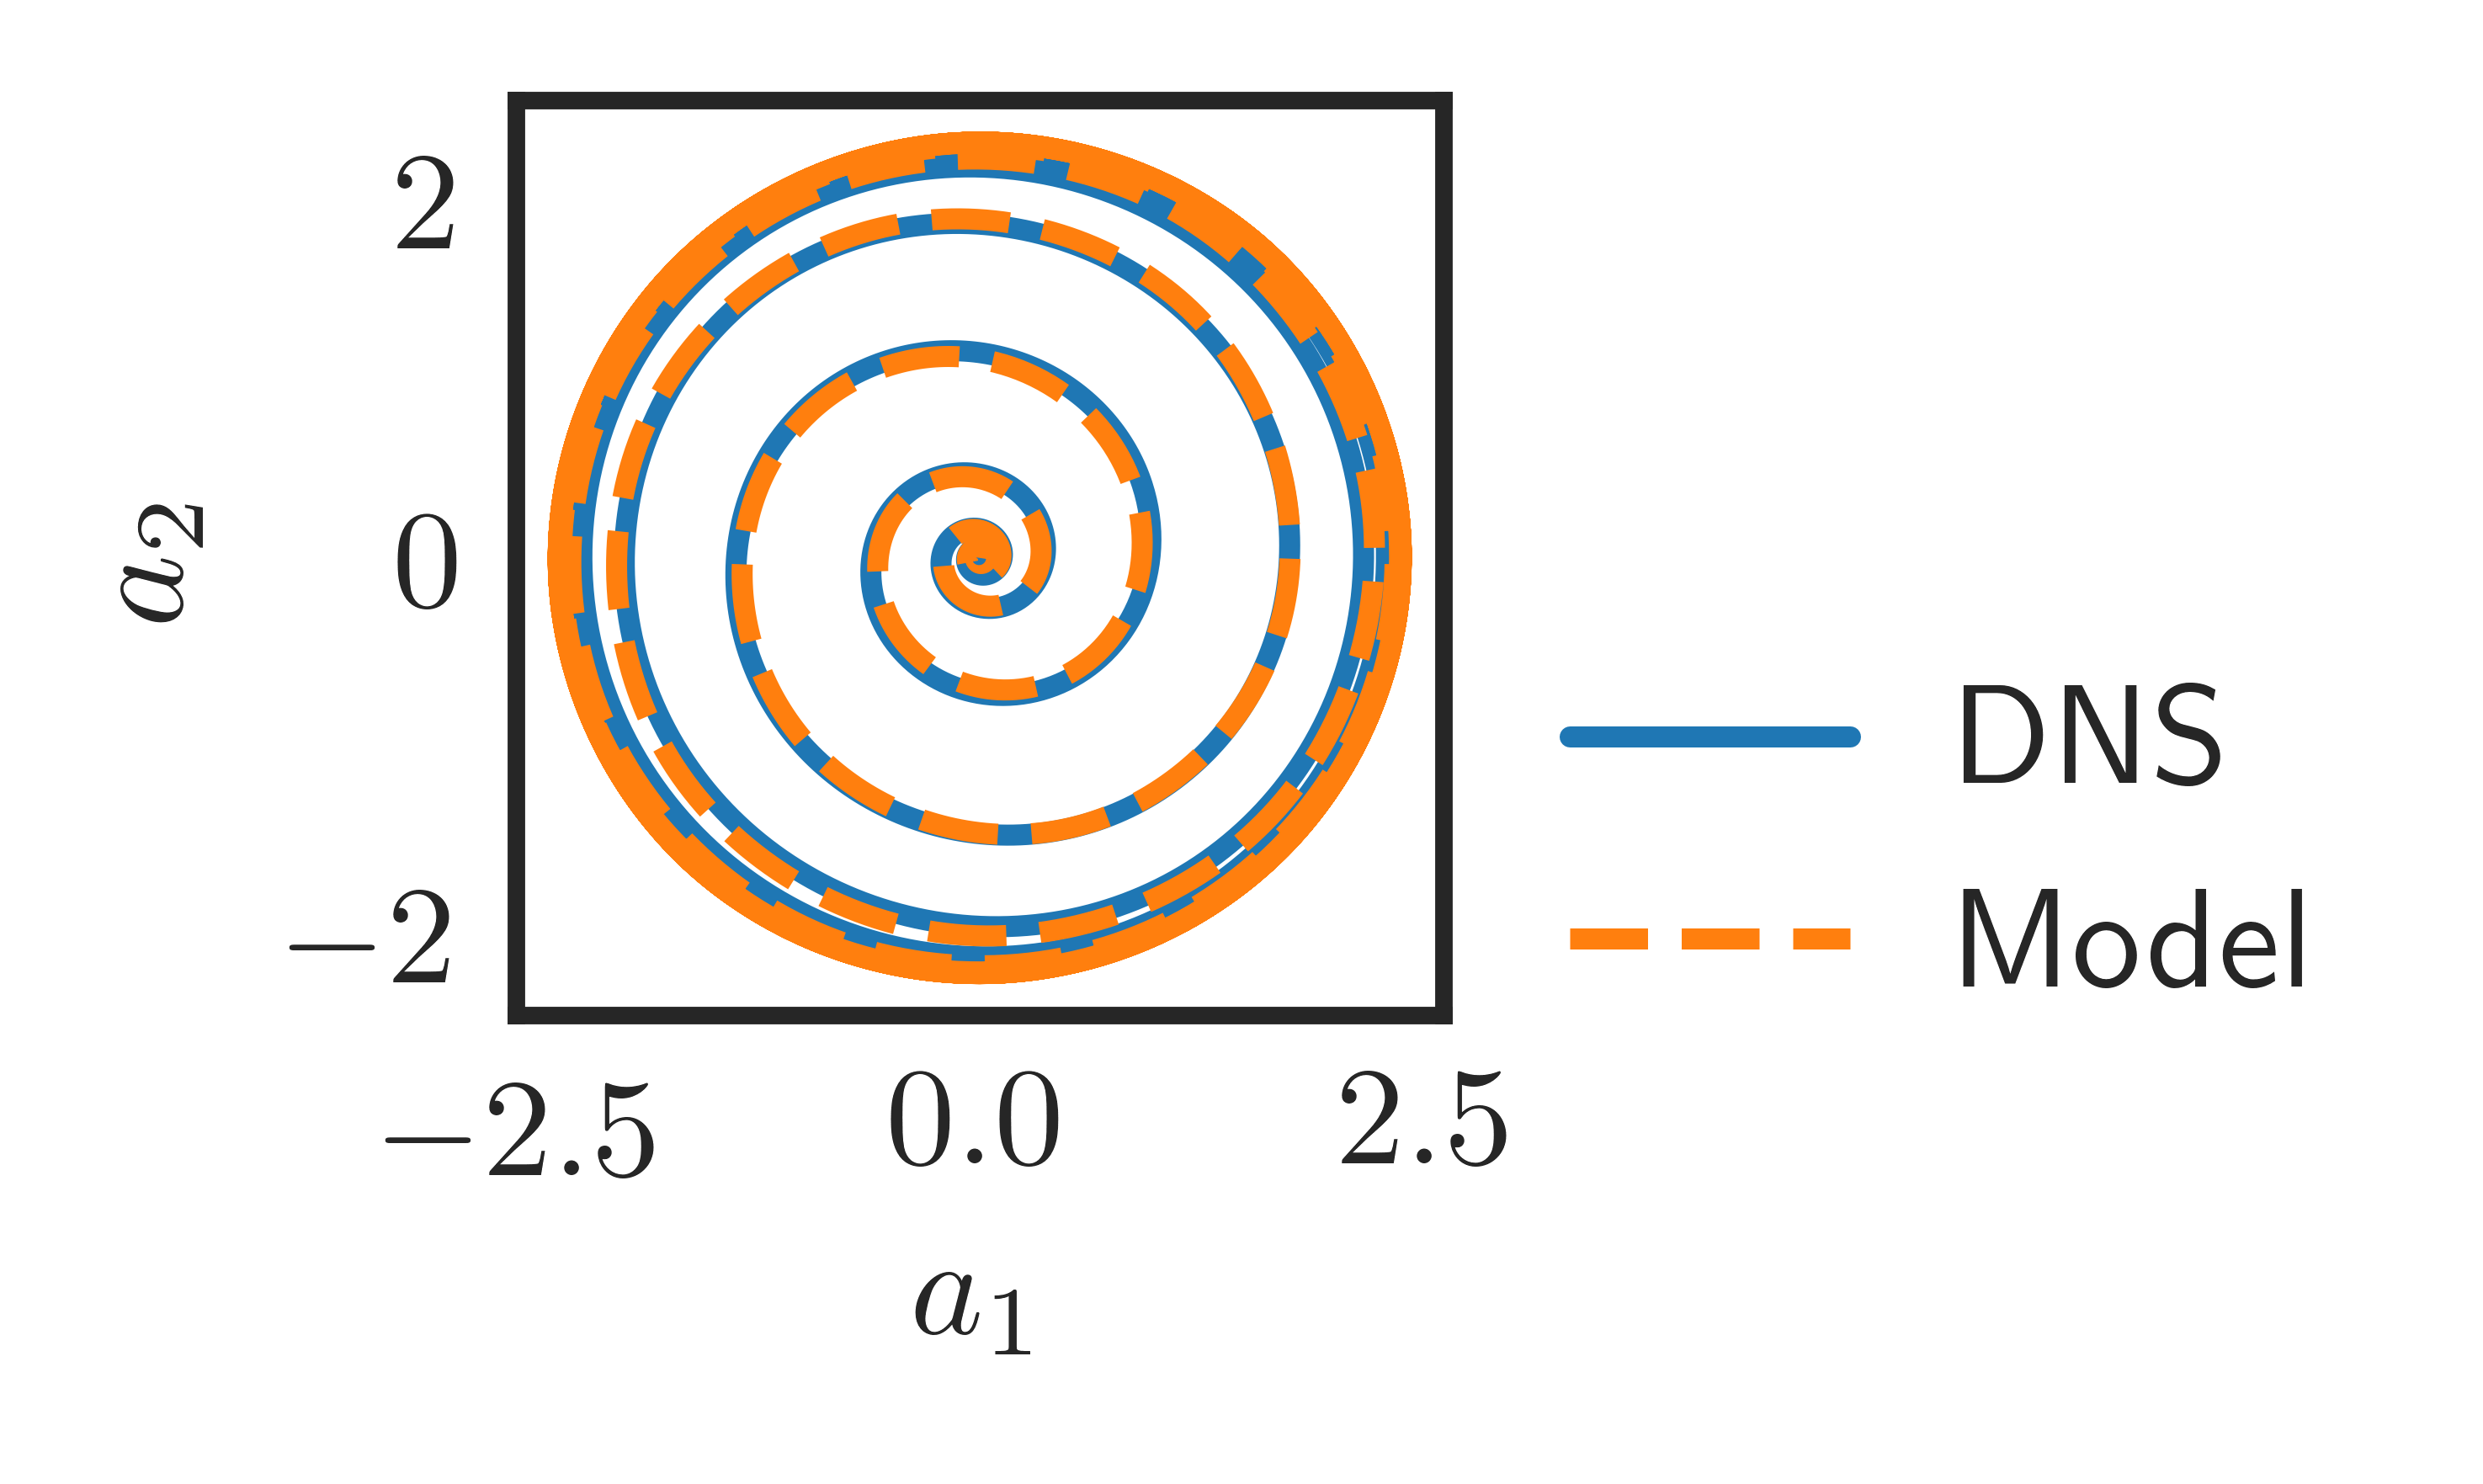
\includegraphics[width=\textwidth]{low_dimensional_phase_plot}
	\end{minipage}

	\vspace{1cm}
\end{frame}

\begin{frame}[t, c]{A gallery of fluid examples}{Low-order \underline{probabilistic} models}
	\begin{minipage}{.38\textwidth}
		\begin{tikzpicture}
			\node[state] (s1) {\( \bm{s}_1 \)};
			\node[state, below right of=s1] (s2) {\( \bm{s}_2 \)};
			\node[state, below left of=s1] (s4) {\( \bm{s}_4 \)};
			\node[state, below left of=s2] (s3) {\( \bm{s}_3 \)};

			\draw (s1) edge[loop above] node {\(l_{11}\)} (s1);
			\draw (s1) edge[bend left] node {\(l_{21}\)}  (s2);

			\draw (s2) edge[loop right]  node {\(l_{22}\)} (s2);
			\draw (s2) edge[bend left]  node {\(l_{32}\)} (s3);

			\draw (s3) edge[bend left]  node {\(l_{43}\)} (s4);
			\draw (s3) edge[loop below]  node {\(l_{33}\)} (s3);

			\draw (s4) edge[bend left]  node {\(l_{14}\)} (s1);
			\draw (s4) edge[loop left]  node {\(l_{44}\)} (s4);

		\end{tikzpicture}
	\end{minipage}%
	\hfill
	\begin{minipage}{.58\textwidth}
		\begin{block}{}
			\centering
			\textbf{Aim :} Identify a \underline{coarse-grain probabilistic} low-order model.
		\end{block}

		\medskip

		\begin{itemize}
			\item Using clustering and symbolic dynamics, a discrete-time probabilistic model can be identified.
			%
			\[
				\bm{p}_{k+1} = \bm{L} \bm{p}_k.
			\]

			\item \textbf{Interpretability :} \( \bm{L} \) describes the transition probability between discrete states \( \bm{s}_i \).

			\medskip

			\item Dynamics are encoded as a probabilistic \underline{finite state machine}.
		\end{itemize}
	\end{minipage}

	\vspace{1cm}
\end{frame}

\begin{frame}[t, c]{Low-order modeling}{Ideal setup}

	\centering

	\begin{tikzpicture}
   	% \draw[help lines](0,0) grid (10,5);

		\node[fill=blue!20, minimum width=1cm, minimum height=3cm, rounded corners, draw=black, thick] (X) at (0, 2.5) {\( \bm{q}_k \)};

		\draw[fill=gray!10, thick] ([xshift=0.75cm]X.north east) -- ([xshift=2.75cm,yshift=0.5cm]X.east) -- ([xshift=2.75cm,yshift=-0.5cm]X.east) -- ([xshift=0.75cm]X.south east) -- cycle;
		\node at (2.25, 2.5) {\textsc{Encoder}};

		\node[fill=gray!10, minimum width=2cm, minimum height=1.0cm, rounded corners, thick, draw=black] (Z) at (5cm, 2.5) {\( \dot{\bm{x}} = \bm{f}(\bm{x}) \)};
		\node at (5, 3.333) {\textsc{Dynamics}};

		\draw[fill=gray!10, thick] ([xshift=0.75cm]Z.north east) -- ([xshift=2.75cm,yshift=1cm]Z.north east) -- ([xshift=2.75cm,yshift=-1cm]Z.south east) -- ([xshift=0.75cm]Z.south east) -- cycle;
		\node at (7.75, 2.5) {\textsc{Decoder}};

		\node[fill=blue!20, minimum width=1cm, minimum height=3cm, rounded corners, draw=black, thick] (Xp) at (10, 2.5) {\( \bm{q}_{k+1} \)};

		\draw[arrow] (X.east) -- ([xshift=0.75cm]X.east);
		\draw[arrow] ([xshift=-0.75cm]Z.west) -- (Z.west);
		\draw[arrow] (Z.east) -- ([xshift=0.75cm]Z.east);
		\draw[arrow] ([xshift=-0.75cm]Xp.west) -- (Xp.west);

	\end{tikzpicture}

	\bigskip

	\begin{block}{}
		\textbf{Ideal setup :} Learn jointly the encoding from the high-dimensional space to the low-dimensional one and the dynamical model within this subspace.
	\end{block}

	\vspace{1cm}
\end{frame}

\begin{frame}[t, c]{Low-order modeling}{In practice}

	\centering

	\begin{tikzpicture}
   	% \draw[help lines](0,0) grid (10,5);

		\node[fill=blue!20, minimum width=1cm, minimum height=3cm, rounded corners, draw=black, thick] (X) at (0, 2.5) {\( \bm{q}_k \)};

		\draw[fill=gray!10, thick] ([xshift=0.75cm]X.north east) -- ([xshift=2.75cm,yshift=0.5cm]X.east) -- ([xshift=2.75cm,yshift=-0.5cm]X.east) -- ([xshift=0.75cm]X.south east) -- cycle;
		\node at (2.25, 2.5) {\textsc{Encoder}};

		\node[fill=gray!10, minimum width=2cm, minimum height=1.0cm, rounded corners, thick, draw=black] (Z) at (5cm, 2.5) {\( \dot{\bm{x}} = \bm{f}(\bm{x}) \)};
		\node at (5, 3.333) {\textsc{Dynamics}};

		\draw[fill=gray!10, thick] ([xshift=0.75cm]Z.north east) -- ([xshift=2.75cm,yshift=1cm]Z.north east) -- ([xshift=2.75cm,yshift=-1cm]Z.south east) -- ([xshift=0.75cm]Z.south east) -- cycle;
		\node at (7.75, 2.5) {\textsc{Decoder}};

		\node[fill=blue!20, minimum width=1cm, minimum height=3cm, rounded corners, draw=black, thick] (Xp) at (10, 2.5) {\( \bm{q}_{k+1} \)};

		\draw[arrow] (X.east) -- ([xshift=0.75cm]X.east);
		\draw[arrow] ([xshift=-0.75cm]Z.west) -- (Z.west);
		\draw[arrow] (Z.east) -- ([xshift=0.75cm]Z.east);
		\draw[arrow] ([xshift=-0.75cm]Xp.west) -- (Xp.west);

	\end{tikzpicture}

	\bigskip

	\begin{block}{}
		\textbf{In practice :} Learning jointly the encoder/decoder and the dynamical model is complicated.
		In practice, they are learned sequentially (i.e.\ first encoder/decoder and then the dynamical model).
	\end{block}

	\vspace{1cm}
\end{frame}

\begin{frame}[t, c]{Our setup for today}{2D Thermosiphon}
  \begin{minipage}{.58\textwidth}
    \begin{itemize}
      \item Two-dimensional flow governed by the incompressible Navier-Stokes equations
      %
      \[
      \begin{aligned}
        \frac{\partial \bm{u}}{\partial t} + (\bm{u} \cdot \nabla ) \bm{u} & = -\nabla p + \textrm{Pr} \nabla^2 \bm{u} + \textrm{Ra Pr } \boldsymbol{\theta} \bm{e}_y \\
        \frac{\partial \boldsymbol{\theta}}{\partial t} + \left( \bm{u} \cdot \nabla \right) \boldsymbol{\theta} & = \nabla^2 \boldsymbol{\theta}.
      \end{aligned}
      \]

      \item \(  Ra  \) and \( Pr  \) are parameters defining our problem.
      \begin{itemize}
        \item[\(  \hookrightarrow \)] \(  Ra  \)   is set to \( Ra = 17\ 000  \).
        \item[\(  \hookrightarrow \)] \(  Pr  \) is set to \( Pr = 5 \).
      \end{itemize}
    \end{itemize}
  \end{minipage}%
  \hfill
  \begin{minipage}{.38\textwidth}
    \centering
    \movie[width=\textwidth, autostart, loop]{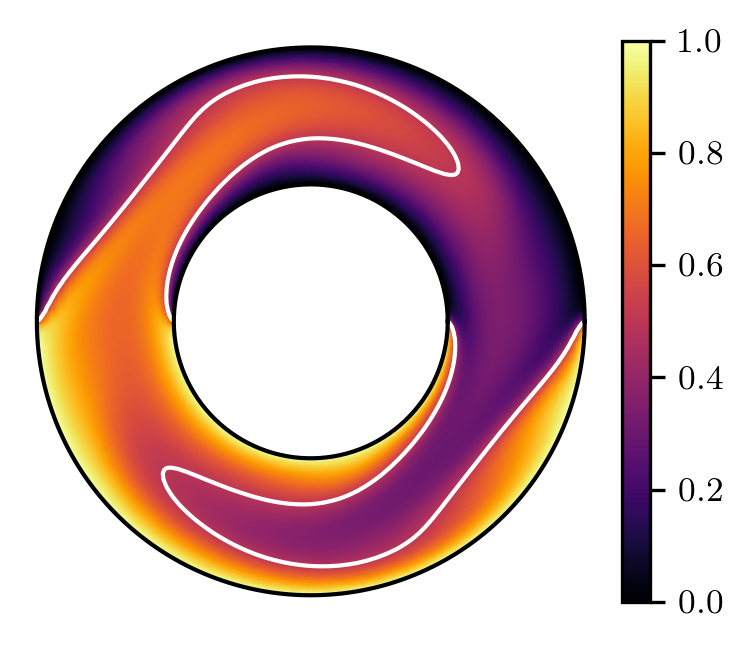
\includegraphics[width=\textwidth]{temperature_field_00000}}{imgs/temperature_evolution.mp4} \\
    {\small
    \textbf{Fig:} Chaotic thermosyphon temp.\ field.
    }
  \end{minipage}

  \vspace{1cm}
\end{frame}

% \begin{frame}[t, c]{2D Thermosiphon}{Chaotic dynamics}
%   \centering
%   % 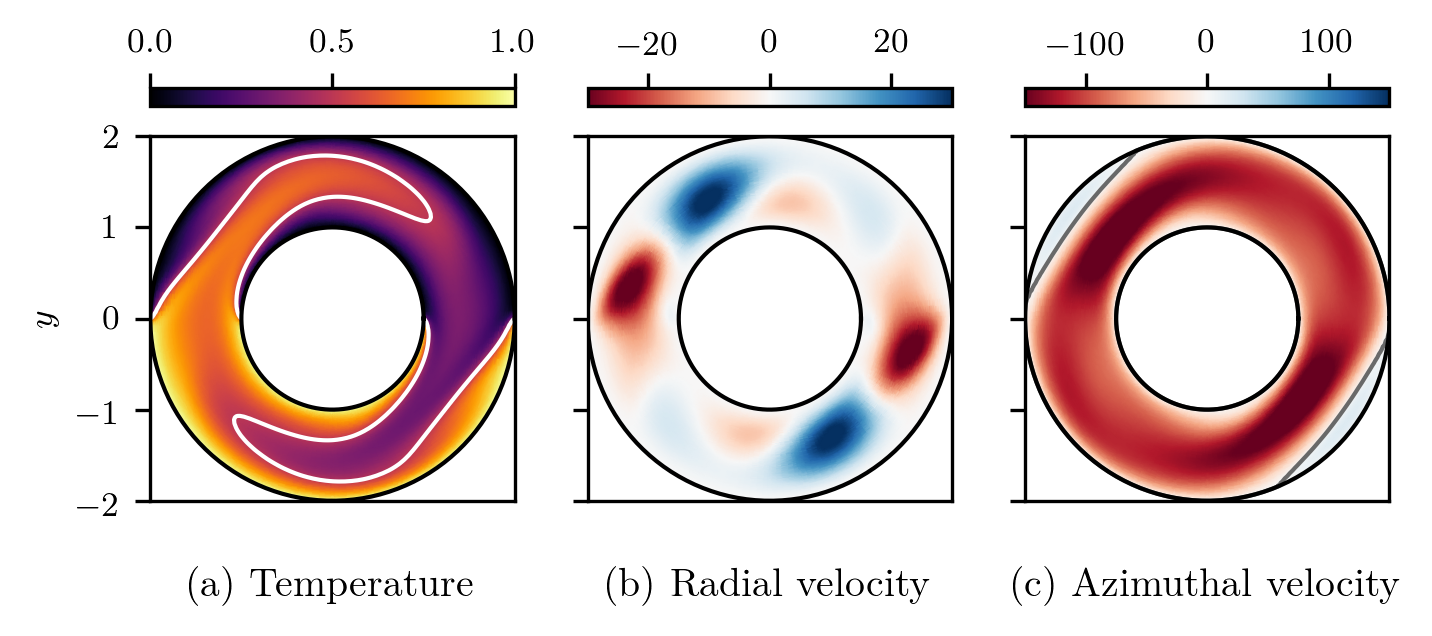
\includegraphics[width=.9\textwidth]{chaotic_thermosyphon_00000}
%   \movie[width=.9\textwidth, autostart, loop]{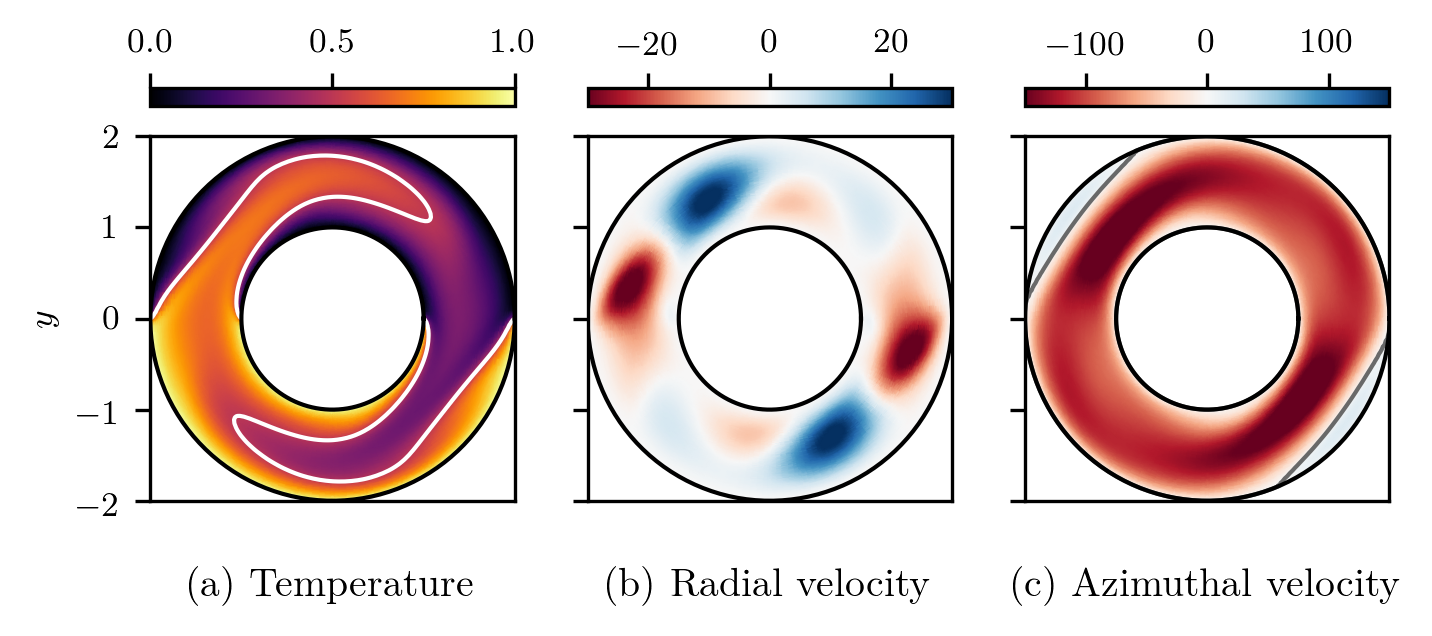
\includegraphics[width=.9\textwidth]{chaotic_thermosyphon_00000}}{imgs/chaotic_thermosyphon.mp4} \\
%
%   \vspace{1cm}
% \end{frame}

\begin{frame}[t, c]{Our setup for today}{Chaotic dynamics}
		\centering
		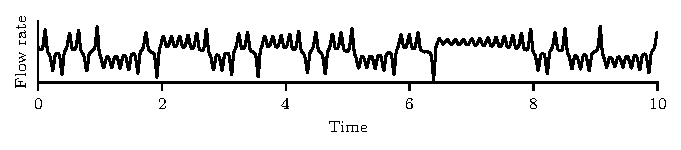
\includegraphics[width=.9\textwidth]{flow_rate_time_series}

		\begin{itemize}
			\item Time-evolution of the cross-sectional flow rate is indicative of Lorenz-like chaotic dynamics.
			\begin{itemize}
				\item[\(	\hookrightarrow	\)] "Random" switching between clockwise and anti-clockwise rotation.
			\end{itemize}

			\medskip

			\item \underline{\textbf{Hypothesis}}: These dynamics can be captured by a low-order model.
		\end{itemize}
  \vspace{1cm}
\end{frame}

\begin{frame}[t, c]{Our setup for today}{A quick detour}
	\begin{minipage}{.58\textwidth}
		\begin{itemize}
			\item Most notorious chaotic dynamical system proposed by Edward Lorenz in 1963.
			It reads
			%
			\[
				\begin{aligned}
					\dot{x} & = \sigma \left( y - x \right) \\
					\dot{y} & = \rho x - y - xz \\
					\dot{z} & = xy - \beta z.
				\end{aligned}
			\]

			\medskip

			\item It can be derived (under certain conditions) directly from the Navier-Stokes equations.
		\end{itemize}
	\end{minipage}%
	\hfill
	\begin{minipage}{.38\textwidth}
		\movie[width=\textwidth, autostart, loop]{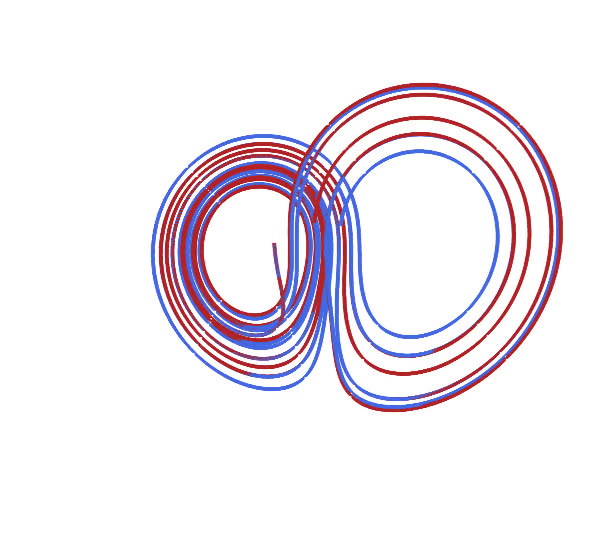
\includegraphics[width=\textwidth]{image_video_lorenz}}{imgs/Lorenz_attractor_JC.mp4}
	\end{minipage}

	\vspace{1cm}
\end{frame}

\begin{frame}[t, c]{Objectives}
  \begin{minipage}{.68\textwidth}
    \begin{itemize}

			\item What physical properties should our reduced-order model have?
			\begin{itemize}
				\item[\(	\hookrightarrow	\)] Analyze the physics prior to modeling.
			\end{itemize}

			\medskip

      \item How to obtain a good low-dimensional embedding?
      \begin{itemize}
        \item[\(  \hookrightarrow \)] Dimensionality reduction.
      \end{itemize}

      \medskip

      \item Can we identify the equations governing the dynamics in the embedded space?
      \begin{itemize}
        \item[\(  \hookrightarrow	\)] System identification.
				\item[\(	\hookrightarrow	\)] How to enforce the physical constraints?
      \end{itemize}

    \end{itemize}
  \end{minipage}%
  \hfill
  \begin{minipage}{.28\textwidth}
		\centering
		
\includegraphics[width=.8\textwidth]{objectives}
  \end{minipage}

  \vspace{1cm}
\end{frame}
